\chapter{MATLAB}

\section{如何遍历当前文件夹及其子文件夹中的全部文件?}

假设现在我们有这样一个文件夹A,它含有一些文件和子文件夹B、C、D......,这些子文件夹又包含若干层子文件夹。我们需要将这个父文件夹(A)及其子文件夹(B、C、D......)和孙文件夹中的所有文件名和其路径取出来。

如果你用的是MATLAB 2016b及更新的版本,那真的太棒了!\codeinline{Matlab}{dir()}函数已经支持遍历搜索了。尝试敲入:

\begin{Matlabcode}
dir_data = dir('**/*');
dir_data([dir_data.isdir]) = [];  % 去除所有.和..文件夹
\end{Matlabcode}

这将会返回一个包含文件信息的struct,现在你可以任意操作这些struct了,随意拼接路径。解放大脑,哦也!方便归方便,但是,一来肯定有大多数人使用的是MATLAB 2016b之前的版本,二来,解放大脑意味着我失去了一次独立思考的机会。

\subsection*{思考}

对于实现方法\footnote{思路来源:\href{https://stackoverflow.com/questions/2652630/how-to-get-all-files-under-a-specific-directory-in-matlab}{How to get all files under a specific directory in MATLAB?}},多层次的遍历,我第一时间想到的是递归。然后就是数据的存储了,\Matlabinline|dir()|函数返回的是一个struct,这个数据结构储存有文件的信息,我们要充分利用这个数据结构。所以现在思路是,写一个递归函数,这个函数返回包含所有文件信息的struct。

这个函数应对先处理父文件夹,获取文件和子文件夹,然后储存文件信息,同时去除子文件夹中的`.'和`..'这两个特殊文件夹。我们对获取的子文件夹再次调用该函数,并储存文件信息。如此,利用递归获取子子孙孙无穷尽文件夹的信息\footnote{其实这并不可能,因为递归是有栈高度限制的,调用函数压入栈,返回函数弹出栈,如果文件夹层次太深,一直压栈就会到达栈溢出警告的极限,例如Python的栈往往是100层,我想MATLAB的栈也大致如此,不会太高},最后函数返回存储有所有文件信息的struct。现在,你可以对这个结构体做你想做的事情。思路如\algoref{get_all_file_name}所示。

\begin{algorithm}[h]
\Function{get\_all\_file\_name(path)}{
    get file and sub\_dir information of current dir\;
    storing file information\;
    remove specific folder of sub\_dir\;
    \For{first sub\_dir \KwTo last sub\_dir}{
        get next sub\_dir\;
        \textbf{recursion} $ \Longrightarrow $ get\_all\_file\_name(path)\;}
    \KwRet{struct of file information}\;
}
\caption{遍历获取当前文件夹及其所有子文件夹中的文件名}
\label{get_all_file_name}
\end{algorithm}

\subsection*{解}

MATLAB 2016b以上的版本我们可以用函数返回struct,这个数据结构包含[folder, name, date, bytes, isdir, datenum]六个字段的信息,我们可以按自己意愿使用folder和name拼接出文件的完整路径。

\Matlabfile[firstline=1]{code/matlab/get_all_file_name_R2016b_newer.m}

MATLAB 2016a及之前的版本dir struct信息并不包含folder,如果返回struct,将只有文件的[name, date, bytes, isdir, datenum]五个字段的信息,所以我们并不能根据函数返回的struct拼接出文件完整路径,\textbf{我们需要自己将路径拼接成一个cell,然后使用函数返回cell}。

\Matlabfile{code/matlab/get_all_file_name_R2016a_older.m}

\subsection*{总结}
\codeinline{Matlab}{dir()}函数遍历整个F盘共2万余文件文件大约需要1.555823s。我们实现的递归函数遍历F盘文件大约需要3.703009s。慢是慢了点,但我们成功运用了递归解决问题,不是吗?

\subsection{如何按自然顺序排序字符串?}

通常,我们会遇到处理一系列文件名有规律的文件的情况,比如:a1.txt、a2.txt ...... a100.txt。但是,当读取文件名到一个cell里后,我们发现文件名往往是乱序排列的,甚至当你使用\codeinline{Matlab}{sort}函数后,排序也不会改变。搜索了一下,在Mathworks File Exchange网站找到了一个自然排序的函数\footnote{\url{https://cn.mathworks.com/matlabcentral/fileexchange/34464-customizable-natural-order-sort}},感谢作者Stephen Cobeldick。效果如下:

\begin{figure}[h]
    \centering
    \begin{minipage}{0.45\textwidth}
        \centering
        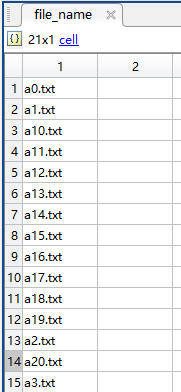
\includegraphics[height=6cm]{disordered_file_name}
        \caption{乱序的文件名}
    \end{minipage}
    \begin{minipage}{0.45\textwidth}
        \centering
        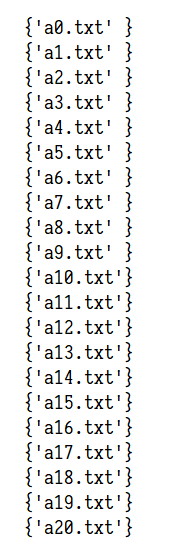
\includegraphics[height=6cm]{ordered_file_name}
        \caption{排序后自然顺序的文件名}
    \end{minipage}
\end{figure}



